\section{基于能量收割的半主动控制磁流变阻尼器}
\subsection{理论模型}
如前所述,结构振动控制作为结构抗震、抗风的核心技术,具有极强的工程需求与研究价值。半主动控制作为结构振动控制中的一类方式,兼具能耗小与智能切换控制状态的优点,是目前最具有工程应用前景的一种结构控制方法。磁流变阻尼器作为一种相对新型的智能阻尼器,具有构造简单,控制能耗低、响应速度快、出力大及可连续调节阻尼等优点,目前也正越来越多地应用于工程领域。结合半主动控制与磁流变(MR)阻尼器无疑为优化结构振动控制提供了一个高效可行的方向。然而,值得注意的是,尽管半主动控制具有能耗小的优点,但其也需要能量输入,同时磁流变阻尼器则是一种典型的直接耗能减振装置,同样也需要一定的能量输入,当其应用于桥梁等户外结构或在地震条件下工作时,不方便或可靠性不能保证的供电,大大制约了半主动控制磁流变阻尼器的应用。事实上,结构减振的过程,就是将结构振动能量耗散的过程,假如将振动的能量收集起来应用于半主动控制磁流变阻尼器的能源供给,上述制约也将迎刃而解。

因此,我们小组设计了一个基于能量收割的半主动控制磁流变阻尼器系统,利用能量收割的原理将振动能量转化为电能供给半主动控制系统与磁流变阻尼器,充分发挥半主动控制与磁流变阻尼器的优势,以达到更优的结构减振效果。系统理论模型如图\ref{system}所示。

\begin{figure}[H]
\bicaption{系统理论模型概念图}{}
\label{system}
\end{figure}

系统工作原理如下:XXXX

由此可见,该系统主要分为MR阻尼器、能量收割模块与半主动控制模块三个部分。由于MR阻尼器的现有研究与工程应用已经相对成熟,我们并未在MR阻尼器的构造上进行过多地创新,仅根据结构特点与需求设计了“双出型”磁流变阻尼器,对其力学性质进行数值模拟与试验测试。针对能量收割模块,我们分析讨论在结构振动控制领域能量收割的一些方式,为验证能量收割的可行性,测算能量转换效率,制作了一个直线型电磁感应能量收割装置进行试验。对于半主动控制模块,XXXX

\subsection{振动能量收割原理及实现方式}

所谓能量收割(Energy Harvesting),是指通过特定方式将通常直接消耗或废弃的能量转化为其他更有用的能量形式。而土木工程结构由于风荷载、地震激励或人致激励产生的振动能就是一种通常直接消耗或废弃的能量,由于结构的振动无所不在,从理论上而言,这种能量非常大,这也意味着土木工程结构能够收割的能量非常大。然而,相对于航天航空、机械、电子等领域的振动能量,土木工程结构的振动能量属于低频能量,往往只有几赫兹,这使得广泛应用于高频能量收割的压电材料并不能够很好地适用于土木工程领域。

目前在土木工程领域已有的能量收割研究主要有两个方向:将振动能量转化为将振动能量转化为液压能与将振动能量转化为电能。由于半主动控制磁流变阻尼器要求的能量输入形式为电能,我们选择的能量收割途径为将振动的机械能转化为电能。静电、压电方式与电磁感应是将振动机械能转化为电能的三种形式,然而由于静电式转换机械能时需要外部电源提供静电场,与我们的目的相悖,而压电式能量转换系统并不能够很好地适用于低频的振动机械能转换。因此,我们选用电磁感应能量转换系统来实现能量收割。

电磁感应能量转换系统,通俗而言,就是应用电磁感应技术进行发电的发电机。电磁感应技术是一项非常成熟,应用发展也非常完善的发电技术。相比于压电能量捕获技术,电磁感应技术电能转换效率更高、发电量更大、理论技术也更为完善,最重要的是,它能够适应土木工程结构低频振动的特点,相对高效地进行结构振动能量收割。目前商用的发电机多为旋转式发电机,但考虑到结构振动是线性运动,如使用旋转式发电机,还需要增加转换装置,制作复杂,也使得机械能耗散加大,降低能量转换效率,所以我们决定根据结构特点,设计直线型发电机用于能量收割。

\subsection{理论最优控制力求解}
线性结构在外部激励和作动器出力的共同作用下,运动方程为
\begin{equation}
\mathbf{M \"{X} + C\.{X} +KX=F(t)+Du} \label{zongfangcheng}
\end{equation}
式中,$\mathbf{K,M,K}$为结构的质量矩阵、阻尼矩阵和刚度矩阵,$\mathbf{F(t)}$为外部激励,$\mathbf{D}$为作动器的位置向量,$\mathbf{u}$为作动器的控制力。

将式\eqref{zongfangcheng}转化为状态方程,令$\mathbf{U=\left(X,\.{X}\right)^T}$,则
\begin{equation}
\dot{\mathbf{U}}=\mathbf{AU+Bu+HF(t)}   \label{zhuangtai}
\end{equation}
式中,

\begin{equation}
\mathbf{
A=\left[
\begin{array}{cc}
0 & I \\
-M^{-1}K & -M^{-1}C
\end{array}
\right],
B=\left[
\begin{array}{c}
0 \\
M^{-1}D
\end{array}
\right],
B=\left[
\begin{array}{c}
0 \\
M^{-1}
\end{array}
\right]
}
\end{equation}

式\eqref{zhuangtai}中,出力结构的状态\textbf{U}未知外,作动器的控制力\textbf{u}同样未知,所以关键是如何得到\textbf{u}.

\subsubsection{经典最优控制}
定义性能指标:
\begin{equation}
\mathbf{min\quad J=\int^{t_f}_0\left[U^T(t)QU(t)+u^T(t)Ru(t)\right]\mathrm{d}t}
\end{equation}
式中,\textbf{Q,R}为权矩阵,分别表示控制效果的权值和控制力的权值。
\begin{equation}
\mathbf{s.t.\quad} \dot{\mathbf{U}}=\mathbf{AU+Bu+HF(t)},\quad \mathbf{U}(0)=\mathbf{U}_0\label{dairu1}
\end{equation}

用优化的方法,可以得到
\begin{equation}
\dot{\mathbf{\lambda}}=\mathbf{-A^T\lambda-2QU,\quad \lambda(t_f)=0}
\end{equation}

\begin{equation}
\mathbf{u=-\frac{1}{2}R^{-1}B^T\lambda}
\end{equation}

方程的解已经在控制工程中得到解决,直接引用结论,作动器控制力为:
\begin{equation}
\mathbf{u=-\frac{1}{2}R^{-1}B^TPU(t)=-GU(t)} \label{konghzhili}
\end{equation}
式中,\textbf{G}称为反馈增益矩阵
\begin{equation}
\mathbf{G=\frac{1}{2}R^{-1}B^TP} \label{fankui}
\end{equation}

将欲求的控制力\textbf{u}再代入式\eqref{dairu1},得
\begin{equation}
\dot{\mathbf{U}}=\mathbf{(A-BG)U+HF(t)}  \label{xianxingjiegou}
\end{equation}

式\eqref{xianxingjiegou}表示一个线性结构,容易求得结构状态\textbf{U(t)}.需要注意的是,在方程求解过程中,忽略了外部激励\textbf{HF(t)},因此只是近似最优。

所以,经典最优控制算法求最优控制力步骤是
\begin{enumerate}
\item 写出结构运动方程,并转化为状态方程\eqref{zhuangtai};
\item 根据式\eqref{fankui},得到反馈增益矩阵\textbf{G};
\item 将\textbf{G}代入式\eqref{xianxingjiegou}求解结构反应;
\item 将结构状态\textbf{U(t)}代入式\eqref{konghzhili},得到作动器的最优控制力。
\end{enumerate}
\subsubsection{瞬时最优控制}
经典最优控制忽略了外部激励 \textbf{HF(t)},所以求得的最优控制力只是近似最优,同时,由于经典的最优控胡子算法的目标函数是一个积分,说明整个时间段内结构参数不变,也就是说,经典最优控制算法只能对线性结构进行求解,为了改进这些问题,Yang 提出了瞬时最优控制算法,该算法作了三点改进:
\begin{enumerate}
\item 性能指标由全部时间内的二次型最小改为每时刻的二次型最小;
\item 不再用 Ricaati 方程求解控制力,而是将状态方程变换为差分方程,差分方程中的变量只与前一时刻的值有关,这样就可以迭代求解控制力和结构的响应;
\item 瞬时最优控制的目标函数是每时刻最优,也就是说,结构仅在微小时段内为线性,所以该算法可以解决非线性结构的控制问题。
\end{enumerate}

首先定义性能指标
\begin{equation}
J=U^T(t)QU(t)+u^T(t)Ru(t)
\end{equation}
状态方程变为
\begin{equation}
U(t)=\Phi d(t-\Delta t)+\frac{\Delta t}{2}\left[Bu(t-)+HF(t)\right]\label{dairu2}
\end{equation}


\begin{equation}
d(t-\Delta t)=e^{\lambda \Delta t}\Phi^{-1}\left\lbrace U(t-\Delta t)+ \frac{\Delta t}{2}\left[Bu(t-\Delta t)+HF(t-\Delta t)\right]\right\rbrace\label{dairu3}
\end{equation}

然后用与经典最优控制算法相同的优化方法,求解得到
\begin{equation}
u=-\frac{\Delta t}{2}R^{-1}B^TQU(t)    \label{kongzhili2}
\end{equation}
再将式\eqref{kongzhili2} 代入式\eqref{dairu2},得
\begin{equation}
U(t)=\left[I+\frac{\Delta t^2}{2}BR^{-1}B^TQ\right]^{-1}\left[\Phi d(t-\Delta t) +\frac{\Delta t}{2}HF(t)\right]  \label{diedai}
\end{equation}

式\eqref{diedai}是一个迭代式,由此可以求得每个时刻的响应。

因此,瞬时最优控制的步骤为:
\begin{enumerate}
\item 写出结构的运动方程,并转化为瞬时的状态方程,如式\eqref{dairu2};
\item 给定结构的初始状态,用式\eqref{dairu3}得到$d(t-\Delta t)$;
\item 按照式\eqref{diedai}得到下一时刻结构的响应$U(t)$;
\item 按照式\eqref{kongzhili2}得到下一时刻的控制力$U(t)$;
\end{enumerate}

%\subsubsection{LQG控制}
%XXXX

\subsection{半主动控制算法及系统}
控制算法选择的好坏直接影响控制系统的性能。对磁流变阻尼结构来货,由于磁流变阻尼器是通过调整磁场的强度来调整产生的阻尼里,接着通过调节事假在磁流变阻尼器的电压(电流)大小使其产生的阻尼里趋向于最优的控制力。有效改变电压(电流)的大小,是利用磁流变阻尼器实现有效控制的关键所在。国内外学者根据磁流变阻尼器的特显,提出了很多种控制策略。

\subsubsection{恒定加压式}
这种控制算法主要包括了 Passive-off, Passive-on 两种形式,分别指对磁流变阻尼器不施加电压和施加最大电压。

在这种恒定加压式控制算法下,磁流变阻尼器相当于一个被动阻尼器,其形式简单,操作便捷,但存在着很大的缺憾:
\begin{enumerate}
\item Passive-off 策略提供的阻尼力较小,不能使磁流变阻尼器发挥出真正的性能。
\item Passive-on 策略提供的阻尼力较大,阻尼器的内力很少有机会超过磁流变阻尼器的屈服力,因此磁流变阻尼器仅起到一个增大结构刚度的作用,未祈祷耗能减振的作用,在地震时因为刚度的增大反而可能加大地震响应。
\end{enumerate}

\subsubsection{离散加压式}
离散加压式指施加在磁流变阻尼器上的电压(电流)的大小分为几个档位,形成双态控制或者三态控制。

常见的双态控制策略一般是当磁流变阻尼器产生的阻尼力小于最优控制力,并且两者方向一致时,将输入电压调到最大,否则为零。

用双态控制对磁流变阻尼器进行控制,计算简单,控制方便,易于操作,但振动较小时容易引起阻尼力超调,使受控结构的动力反应产生局部放大的现象,引起负面效应。

为此有人提出了三态控制,控制档位增设中间一档,但虽然优于双态控制,但仍然未发挥磁流变阻尼器全部性能,控制策略仍然不够细腻。

\subsubsection{PID控制}

PID控制是比例(P)、偏差积分(I)、偏差微分(D)控制的简称。常规PID控制系统原理孔图如图所示 XXXX


\paragraph{PID控制基本原理}
\qquad 控制规律为
\[\mathrm{u}(t)=\mathrm{MV}(t)=K_p{e(t)} + K_{i}\int_{0}^{t}{e(\tau)}\,{d\tau} + K_{d}\frac{de(t)}{dt}\]

其中:
$K_p$:比例增益,是调适参数\\
$K_i$:积分增益,也是调适参数\\
$K_d$:微分增益,也是调适参数\\
$e$:误差=设定值(SP)- 回授值(PV)\\
$t$:目前时间\\
$\tau$:积分变数,数值从0到目前时间t

\paragraph{PID控制器设计及参数整定}
\qquad 采用PID控制策略时,$K_{k},K_{i},K_{p}$三个参数对系统的控制效果起决定性作用,采用凑试发确定 PID参数,分为以下几步:
\begin{enumerate}
\item 首先选择 $K_p$ 值得到期望的暂态响应,而置 $K_i,K_d$为零,然后逐步改变 $K_p$,同时观察系统变化,知道控制系统得到响应较好,超调小的响应曲线。此时系统仍有较大的稳态误差。
\item 加入积分环境,整定积分参数。首先置$K_i$为一个较小的值,同时变化$K_p$为较小值,不断变化$K_i$,使系统在保持良好动态性能的情况喜爱,静差得到消除。
\item 加入微分环节,构成PID控制器,微分系数$K_d$的整定方法同第二步,逐步增大$K_d$的同时相应地变化$K_p,K_i$,逐步试凑,以获得满意的调节效果和控制参数。
\end{enumerate}

%\paragraph{PID控制仿真结果}


\subsubsection{模糊控制}
磁流变阻尼器双态控制和三态控制电流的选择档次只有两档和三档,控制较为粗糙,想要实现精确地控制加入磁流变阻尼器的结构,最好实行全态控制。

为了在短暂的时间内实现全态的励磁电流选择,将模糊逻辑控制技术应用到加入磁流变阻尼器结构的全态控制中,即采用模糊逻辑控制器根据传感器所采集的机构状态信号和外界激励信号瞬时作出电流选择,所确定的电流输入到阻尼器实现对结构的全态控制。

如图 XXXX,每一时刻地震加速度和建筑结构的状态被信号检测器检测并被输入到模糊逻辑控制器中,在预定的模糊规则和隶属函数下经模糊逻辑控制器的模糊推理后,得到一控制电流,将控制电流指令信号传递给磁流变阻尼器,磁流变阻尼器产生控制力并施加给结构。这便是加有磁流变阻尼器结构的模糊逻辑全态控制的整个构思框架。

\paragraph{输入量、输出量的选取}
\qquad 模糊控制器应用比较多的是以误差和误差的变化为输入变量的二维模糊控制,选用位移与系统位移响应之间的误差$e$ 与变化率$\Delta e$作为控制器的输入量,控制电流变化的量为输出。
\paragraph{输入、输出变量的正规化处理及基本论域确定}
\qquad 在模糊控制器设计中,信号的实际变化范围称为变量的基本论域,误差变化及输出变量的变化区间,经变换得到正规化输入输出变量为:
\[x=\frac{e}{e_{max}}\qquad \qquad y=\frac{\Delta e}{\Delta e_{max}}\qquad \qquad z=\frac{I}{I_{max}}\]

其中,$x\in [-1,1]; y\in [-1,1]; z\in [0,1]$.

\paragraph{模糊集合与隶属函数的确定}
\qquad 对论域 $x,y$,定义五个模糊子集表示输入的模糊状态
\[\mathbf{\lbrace NB,NS,Z,PS,PB\rbrace}\]
输出变量$z$的模糊集合也定义五个子集表示
\[\mathbf{\lbrace Z,S,M,SB,B\rbrace}\]
模糊语言变量隶属度函数输入、输出采用高斯型如图
\begin{figure}[H]
\centering
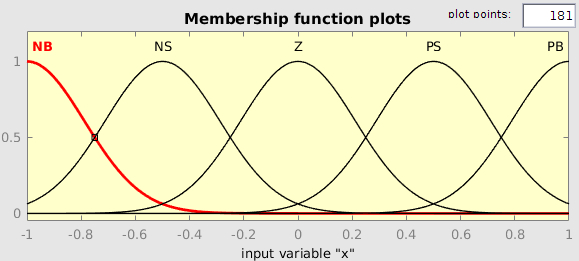
\includegraphics[width=0.5\linewidth]{figure/fuzzyx}
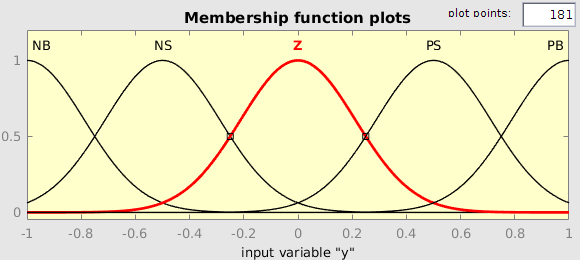
\includegraphics[width=0.5\linewidth]{figure/fuzzyy}
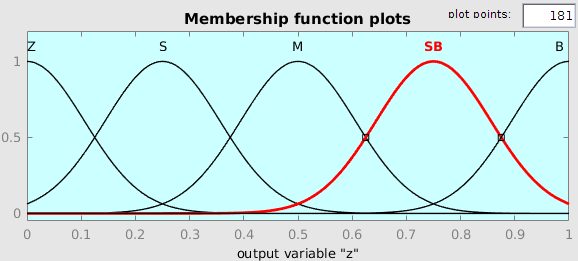
\includegraphics[width=0.5\linewidth]{figure/fuzzyz}
\end{figure}

\paragraph{模糊控制规则的确定}
\qquad 模糊控制规则采用相关参考文献的控制规律 XXXX,根据模糊推理规则,输出与位移变化及其变化率的曲面关系如图XXXX
\begin{figure}[H]
\centering
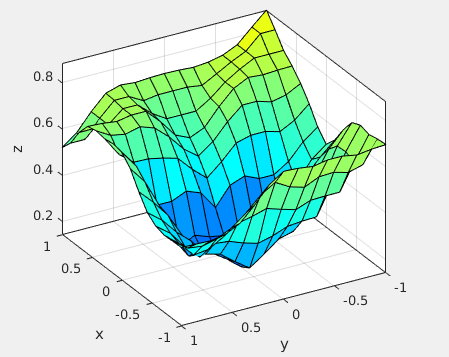
\includegraphics[width=0.5\linewidth]{figure/fuzzysurface}
\end{figure}

\paragraph{模糊推理与去模糊化}
\qquad 模糊推理本质上是将一个给定输入空间通过模糊逻辑的方法映射到一个特定的输出空间的计算过程。模糊控制器选择 Mamdani 推理法。经模糊控制器算出的精确控制量,通过输出控制量的比例因子确定输出的控制电流信号。采用重心法去模糊化。下图给出了一个该模糊控制器的推理实例:

\begin{figure}[H]
\centering
\bicaption{$x=-0.3,y=0.7$时,模糊推理器的推理过程}
{When $x=-0.3,y=0.7$}
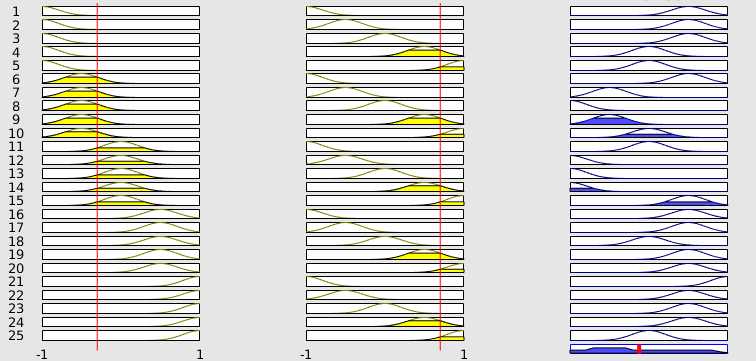
\includegraphics[width=0.5\linewidth]{figure/fuzzyeg}
\end{figure}

%\paragraph{模糊控制仿真}
%\qquad

%\subsubsection{天棚阻尼}
%

\subsection{实验模型设计}

\subsection{优势与创新}

\subsubsection{半主动控制,效果与稳定兼顾}
我们提出的基于磁流变阻尼器的结构振动控制系统属于半主动控制系统。一方面,半主动控制系统能够在更大的地震动卓越频率范围内发挥作用,克服了被动控制系统调节范围窄的缺点;另一方面,半主动控制系统对外界的能量输入依赖小,克服了主动控制系统能量输入大、系统可靠性低的弊端。

\subsubsection{磁流变液,出力效率高}
磁流变液是诞生于上世纪50年代的一种智能材料,近年来,磁流变液在工程领域的应用日益丰富,但其应用主要集中在机械工程、汽车工程领域,我们创新性地将其应用在建筑结构的抗震方向。与传统的建筑结构抗震设备相比,以磁流变液为阻尼材料的阻尼器能够以更小的质量与体积输出更大的阻尼力,从而节省建筑空间、减轻结构自重。更为重要的,磁流变液的响应时间短,使结构振动的实时控制成为可能。

\subsubsection{自主供能,因地制宜}
基于上文的讨论,我们可以根据建筑的场地环境、结构体系以及受力特点,因地制宜地选择太阳能发电、压电转换、风力发电等一系列发电机制,进而实现整个控制系统的自主供能。自供能的实现一方面有利于减少能源消耗,降低系统的维护成本,更为重要的,是使整个系统摆脱了是使整个系统摆脱了对外部能源的依赖,有利于保证系统在地震等灾害环境下依然能够发挥控制结构振动的作用。

\subsubsection{子系统模块化,易于更新}
在我们建立的理论模型中,我们有意识地将各个子功能模块化,即发电模块、传感器输入模块、控制算法模块、响应输出模块,各个子系统通过标准接口进行信息传递。这种设计除了使整个系统结构清晰、简便易行之外,模块化的功能封装使得各个子系统都能够根据相应领域的技术发展进行更近迭代,始终保持整个系统的高效运转。

\subsubsection{嵌入式系统,提高系统可靠度}
与传统的主动控制、半主动控制系统借助计算机实现控制算法相区别,我们选择在可编程硬件上进行算法的设计编程,也即上文论述的理论模型是一个嵌入式系统。在我们的嵌入式系统中,控制算法硬件与阻尼器融为一体,克服了在灾害条件下计算机可能无法正常工作、通讯故障的潜在风险,提高了控制系统的可靠度。